\documentclass[journal,onecolumn]{IEEEtran}
%\usepackage[letterpaper,margin=1in]{geometry}
\usepackage[english]{babel}
\usepackage[utf8]{inputenc}
\usepackage{fancyhdr}
\usepackage{mathtools}
\usepackage{amsmath}
\usepackage{amssymb}
\usepackage{textcomp}
\usepackage[table,xcdraw]{xcolor}
\usepackage{cite}
\usepackage{float}
\usepackage{csquotes}
\usepackage{verbatim}
\usepackage{url}
\usepackage{listings}
\usepackage{color}

\definecolor{codegreen}{rgb}{0,0.6,0}
\definecolor{codegray}{rgb}{0.5,0.5,0.5}
\definecolor{codepurple}{rgb}{0.58,0,0.82}
\definecolor{backcolour}{rgb}{0.95,0.95,0.92}

\lstdefinestyle{mystyle}{
	backgroundcolor=\color{white},   
	commentstyle=\color{codegreen},
	keywordstyle=\color{black},
	numberstyle=\tiny\color{codegray},
	stringstyle=\color{codepurple},
	basicstyle=\footnotesize,
	breakatwhitespace=false,         
	breaklines=true,                 
	captionpos=b,                    
	keepspaces=true,                 
	numbers=left,                    
	numbersep=5pt,                  
	showspaces=false,                
	showstringspaces=false,
	showtabs=false,                  
	tabsize=2,
	frame=leftline
}

\lstset{style=mystyle}
%opening
\title{ECE 2060 Lab 1\\ 
\Large \textit{Introduction to Lab Equipment}}
\author{Matt Gambill ~\IEEEmembership{Member, OSU IEEE} \\
		Hamzah Khan\\
		Sky Mandava}
% \date{\today}

\begin{document}

\maketitle

\begin{abstract}
This lab served as a practical to familiarize students with the instruments that Electrical and Computer Engineers use to test their designs. Students learned how to use a signal generator, oscilloscope, power supply, and Quartus FPGA software.
\end{abstract}

\section*{Introduction}
Near the beginning of the semester at The Ohio State University Department of Electrical and Computer Engineering (ECE). Students in ECE 2060 Digital Design get a refresher or primer on how to use Laboratory Equipment. Students will be using the Equipment throughout the semester to measure various signals so the primer/refresher is welcome. In this paper I introduce some of the data that came from playing around with the equipment, and some of the screenshots from the oscilloscope.
\section*{Procedure and Results}
Students gathered the supplies they needed.\footnote{ See \cite{readMe} the for a list of supplies used and a detailed procedure.} 
There are two parts to the lab. Part I explores operation of the oscilloscope and function generator. The function generator was set to 1.000 kHz, Peak to Peak Voltage of 2 Volts and a Duty Cycle of 30\%.
 
Here is a screenshot from the oscilloscope measuring the function generator's signal:
\begin{figure}[H]
	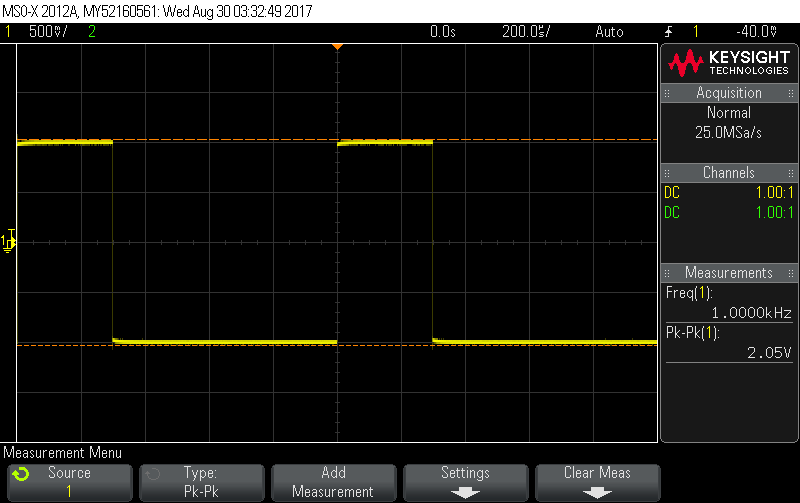
\includegraphics[width=18cm]{functionGenerator_2.png}
	\centering
	\caption{Function Generator Screenshot}
	\label{fig:fgs}
\end{figure}
\newpage
Figure \ref{fig:fgs} data has been summarized in Table \ref{tab:fg}
\begin{table}[H]
	\centering
	\caption{Function Generator Data}
	\label{tab:fg}
	\begin{tabular}{|l|c|c|}
		\hline
		\textbf{Measurement} & \textbf{Value} & \textbf{Units}           \\ \hline
		\rule{0pt}{4ex}  Horizontal Sweep     & 200            & $\frac{\mu s}{division}$ \\ \hline
		\rule{0pt}{4ex}  Vertical Sweep       & 500            & $\frac{mV}{division}$    \\ \hline
		\rule{0pt}{4ex}  Peak to Peak Voltage & 2.05           & Volts                    \\ \hline
		\rule{0pt}{4ex}  Frequency            & 1.0000         & kHz                      \\ \hline
	\end{tabular}
\end{table}
The data was written into a csv and plotted in Matlab with plotData.m.
\lstinputlisting[language=Octave]{plotData.m}
\begin{figure}[H]
	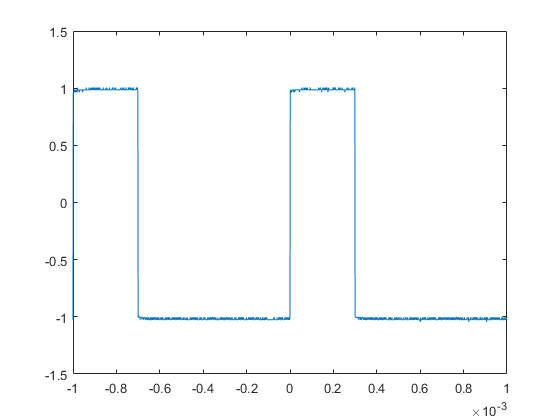
\includegraphics{OscilloscopeDataPlot.png}
	\centering
	\caption{Function Generator Data Plot}
	\label{fig:fgdp}
\end{figure}

In Figure \ref{fig:fgdp} you'll notice some noise on logical high and logical low, this is expected.

The next activity was to measure the output of pin 1 on a FPGA board. First measured with the probe the screen looked like Figure \ref{fig:srpb} and data summarized in Table \ref{tab:FPGA_APrb}.
\begin{figure}[H]
	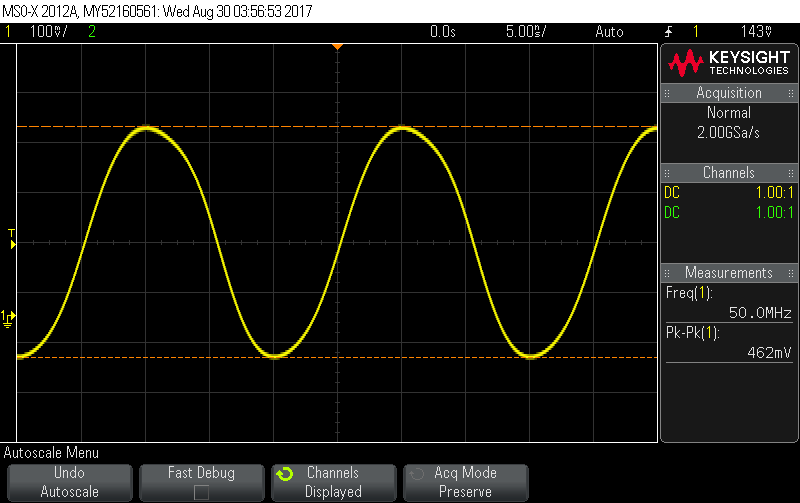
\includegraphics[width=18cm]{probe_sine.png}
	\centering
	\caption{FPGA Analog Probe}
	\label{fig:srpb}
\end{figure}
\begin{table}[H]
	\centering
	\caption{FPGA Analog Probe Data}
	\label{tab:FPGA_APrb}
	\begin{tabular}{|l|c|c|}
		\hline
		\textbf{Measurement} & \textbf{Value} & \textbf{Units}                        \\ \hline
		\rule{0pt}{4ex}  Horizontal Sweep     & 5.00            & $\frac{ns}{division}$ \\ \hline
		\rule{0pt}{4ex}  Vertical Sweep       & 100            & $\frac{mV}{division}$  \\ \hline
		\rule{0pt}{4ex}  Peak to Peak Voltage & 462            & mV                      \\ \hline
		\rule{0pt}{4ex}  Frequency            & 50.0           & MHz                      \\ \hline
	\end{tabular}
\end{table}
\newpage
The analog probe was then switched to a bnc to header adapter. Data is summarized in Table \ref{tab:FPGA_BPrb}.
\begin{figure}[H]
	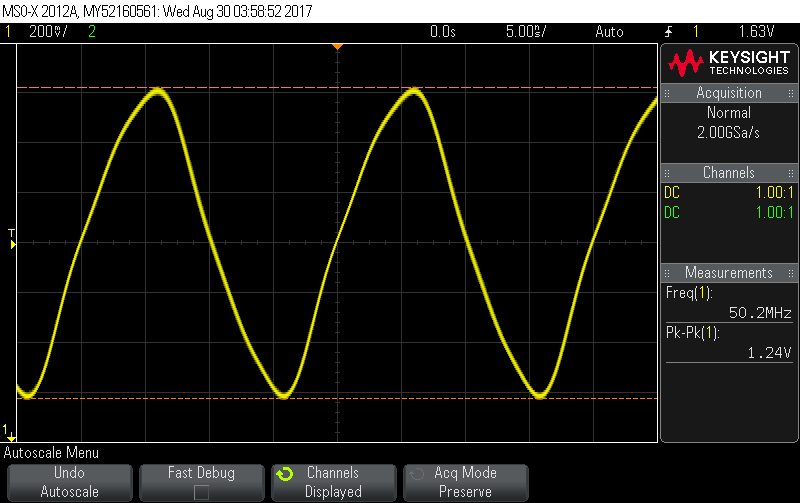
\includegraphics[width=18cm]{bnc_sine.png}
	\centering
	\caption{FPGA BNC Probe}
	\label{fig:sbnc}
\end{figure}
\begin{table}[H]
	\centering
	\caption{FPGA BNC Probe Data}
	\label{tab:FPGA_BPrb}
	\begin{tabular}{|l|c|c|}
		\hline
		\textbf{Measurement} & \textbf{Value} & \textbf{Units}                        \\ \hline
		\rule{0pt}{4ex}  Horizontal Sweep     & 5.00           & $\frac{ns}{division}$ \\ \hline
		\rule{0pt}{4ex}  Vertical Sweep       & 200            & $\frac{mV}{division}$  \\ \hline
		\rule{0pt}{4ex}  Peak to Peak Voltage & 1.24           & Volts                   \\ \hline
		\rule{0pt}{4ex}  Frequency            & 50.2           & MHz                      \\ \hline
	\end{tabular}
\end{table}
\newpage
The probe was then switched out for the digital probe with results in Figure \ref{fig:FPGA-D}.
\begin{figure}[H]
	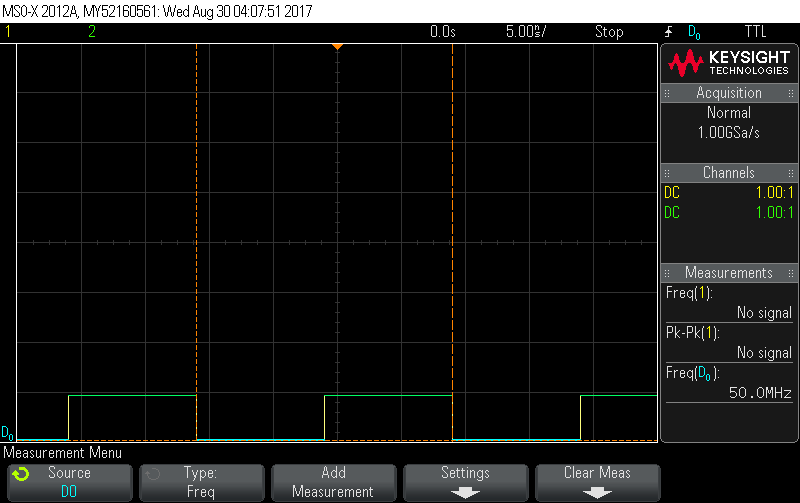
\includegraphics[width=18cm]{digital_2.png}
	\centering
	\caption{FPGA Digital Probe}
	\label{fig:FPGA-D}
\end{figure}
In Figure \ref{fig:FPGA-D} we observe a 50.0 MHz duty cycle.



\section*{Discussion}
The horizontal units on the oscilloscope are either nanoseconds or microseconds per division. You can change the setting by turning a knob near the top left of the oscilloscope called the "Horizontal Knob." The setting can be read near the top of the screen.

The Vertical Units on the oscilloscope are Volts or mV per division. You change the setting by turning the Vertical Amplifier knob. The setting can be read in the top right corner of the oscilloscope's screen.

The equation for period is $T = \frac{1}{f}$. With a 50MHz frequency the period is $T = \frac{1}{50\times 10^6}$ or 20 nanoseconds.

Comparing Figure \ref{fig:srpb} to Figure \ref{fig:FPGA-D} we see the the digital signal is much cleaner than the analog signal. This digital signal will be more useful for digital logic.
\section*{Conclusion}
Technically all signals are analog, however one way to think about digital signals is that they are the first abstraction needed to do logic and computation. The goal of the lab was to gain experience with lab equipment and present some simple measurements, so there isn't a whole lot to conclude; however in later papers I'll present some more findings that will more interesting to the academic community.
\section*{Acknowledgements}
I'd like to thank Sky and Hamann for their help in Lab.
\bibliographystyle{IEEEtran}
\bibliography{IEEEabrv,References}




\end{document}
